%------------------------------------------------------------------------------
\section{Experimental Methods}
\label{ch:exp}

The experimental data analysed in this chapter was acquired by Xing Chen, under the supervision of Alexander Thiele at the Institute of Neuroscience, Newcastle University.
All procedures were carried out in accordance with the European Communities Council Directive RL 2010/63/EC, the US National Institutes of Health Guidelines for the Care and Use of Animals for Experimental Procedures, and the UK Animals Scientific Procedures Act. Two male macaque monkeys (5 and 14 years of age) were used in this study.


\subsection{Head post implantation}

During an initial surgical operation, a custom-made head post (Peek, Tecapeek) was embedded into a dental acrylic head stage.
Details of the surgical procedures and post-operative care have already been published \citep[see][]{Thiele2006}.


\subsection{Stimuli}

Stimuli were displayed on a \ac{CRT} monitor with display dimensions \SI{400x320}{\milli\metre} at a viewing distance of \SI{0.54}{\metre}, with resolution \SI{1280x1024}{px}.
The monitor refresh rate was \SI{85}{Hz} for \ac{M1} and \SI{75}{Hz} for \ac{M2}.


\subsection{Initial training}

The monkeys were familiarised with the experimental set-up and structure with an initial training task otherwise unrelated to the main perceptual learning task on which the animals were later trained.
In this initial task, the animals compared the colour of a circle stimulus with that of succeeding circle stimuli, while maintaining fixation on a central target.
When a target stimulus appeared (a circle of a matching colour), subjects were required to release a touch bar in order to receive a fluid reward.
Eye position was monitored using an infrared video tracking system.% (Dalsa CCD camera, model SIM-0002, and eye-tracking software from Thomas Recording ET-49 --- Version 1.2.8).


\subsection{Electrode array implantation}

During surgery, animals were sedated with ketamine, and general anaesthesia was maintained using isoflurane following endotracheal intubation.
% Heart rate, respiratory rate, blood pressure, \ac{ECG}, \ce{O2} saturation, expiratory \ce{CO2}, and skin and rectal body temperature were monitored continuously during the operation.
% Fluids and antibiotics were administered intravenously.
% The animals were placed in a stereotaxic head holder and the skull overlying the occipital and posterior temporal cortices was exposed.
A craniotomy was made to remove the bone overlying \ac{V1}, V2, and dorsal \ac{V4}, using a pneumatic drill.
The bone was kept in sterile 0.9\% \ce{NaCl} for refitting at the end of the surgery.
The dura was opened up to allow access to regions \ac{V4} and \ac{V1}.
Microelectrode chronic Utah arrays, attached to a CerePortTM base, were implanted under sterile conditions in the cortex.
%, using a Blackrock microarray inserter.
For \ac{M1}, two $4{\times}5$ grids of microelectrodes were implanted in area \ac{V4}, and one $5{\times}5$ grid was implanted in \ac{V1}.
For \ac{M2}, a $5{\times}5$ grid was implanted in \ac{V4}, and a $5{\times}5$ grid in \ac{V1}.
% The electrode contacts within each \ac{MEA} had a separation distance of XXX, which is sufficiently distant from each other such that neurons can be close enough at most one electrode contact for their spiking activity to be detected.
% Wire bundles were held in place with biologically-compatible glue (histoacrylic), and the connector (CerePortTM) was secured to the skull with titanium bone screws.
% In both animals, the titanium screws were rejected by the bone within 6 to 10 weeks following the implant, so a dental acrylic bridge was built to fuse the base of1 the connector to the existing head stage, during a subsequent surgical operation.

As is common with intricate electrical work, a minority of electrode contacts were unstable and post-surgery were found to have high impedance.
These electrodes (channels) were not viable for use in electrophyisiological recordings.
The number of recording channels from the \acp{MEA} used in the study are shown in \autoref{tab:nchannels}.

\begin{table}[bthp]
\caption{Number of channels recorded from for each of the monkeys and brain regions.}
\label{tab:nchannels}
\begin{center}
\begin{tabular}{ccr}
\toprule
Animal  & Region    & Number of viable channels \\
\midrule
M1      & V4        & 30 \\
        & V1        & 23 \\
M2      & V4        & 20 \\
        & V1        & 25 \\
\bottomrule
\end{tabular}
\end{center}
\end{table}


\subsection{Receptive fields}

After animals had fully recovered, \acp{RF} were mapped using reverse correlation between random stimulation and neuronal response.
For both animals, the \acp{RF} of neurons recorded from the \ac{V4} arrays were \SI{7.5}{\degree} from the centre of the visual field.
For \ac{M1}, the \ac{MEA} in \ac{V1} was \SI{4.6}{\degree} from the centre, and for \ac{M2} it was \SI{1.5}{\degree}.
In macaques, the foveal region spans \SI{\pm1}{\degree} from the centre of vision.
% (Hanazono, Tsunoda, Kazato, Suzuki, & Tanifuji, 2012)
Thus, every \ac{MEA} corresponded retinotopically to the parafoveal region of the visual field.

Since the effects of perceptual learning are restricted to neurons which encode the training stimulus, the experimental protocol was performed for stimuli located in the \ac{V1} and \ac{V4} locations separately.


\subsection{Behavioural task}

Consequently, the experimental procedure was performed twice for each animal, first with stimuli located within the visual field so as to stimulate the neurons recorded from the \ac{V4} implant, and then for the \ac{V1} implant.

The experimental design has been described previously \citep[see][]{Chen2013}.
Briefly, the experiment comprised 4 stages, illustrated in \autoref{fig:pltask1}, each of which conform to the same overarching structure.
Each experiment is composed of a series of trials.
On each trial, the monkey must first fixate their gaze on a fixation point, which is a black cross on a grey background with \SI{50}{\percent} contrast displayed on a monitor in front of the monkey.
For \ac{M1}, the refresh rate of the monitor was \SI{85}{Hz}, whilst for \ac{M2} it was \SI{75}{Hz}.

\begin{figure}[htbp]
\begin{center}
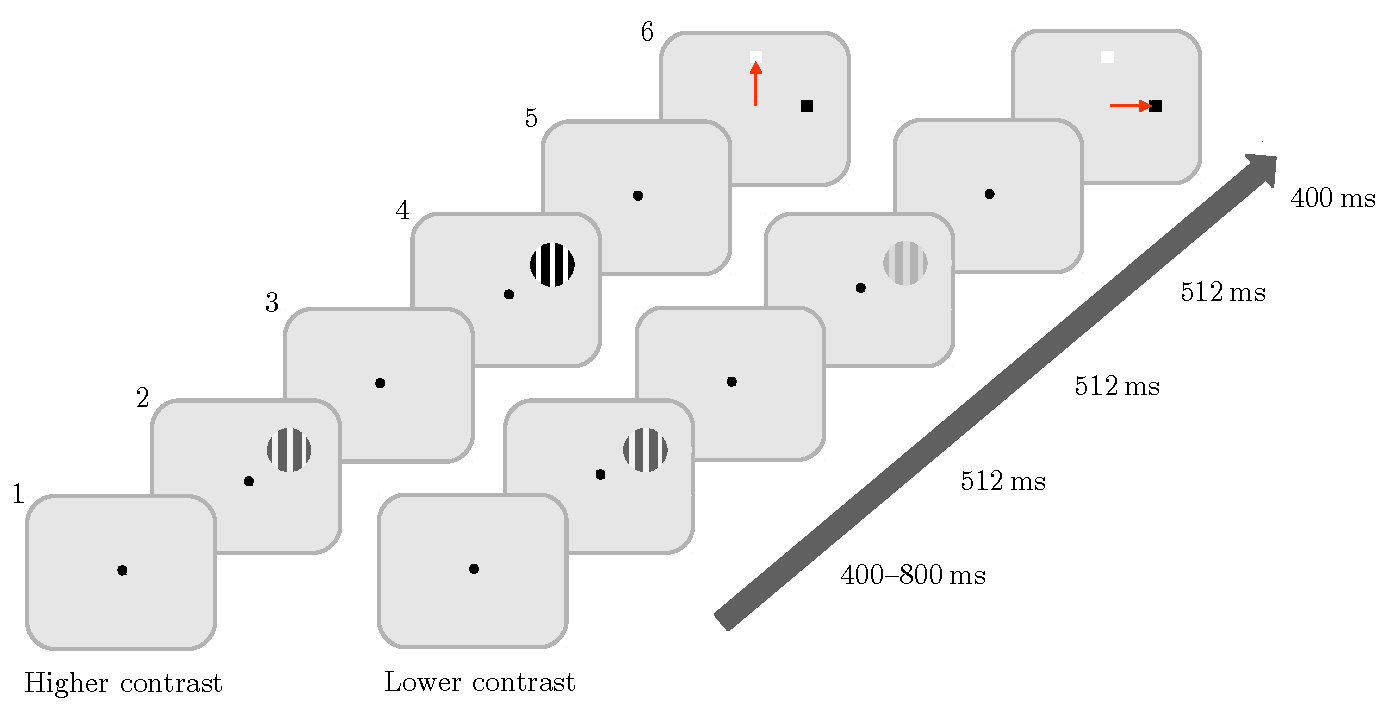
\includegraphics[width=\linewidth]{figs/task/PLtask1.pdf}
\end{center}
\caption{
Experimental procedure.
1:~The monkey fixates upon a central spot.
2:~A sample stimulus in the form of either a Gabor patch or a sine grating is presented at the pedestal contrast (\eg{}~\SI{30}{\percent}).
3:~Blank sample-test interval.
4:~Test stimulus presented.
5:~Blank test-target interval.
6:~Two target stimuli appear to the left and right of the test stimulus location, signalling that the subject is allowed make a saccade to their chosen target.
Subject's overall objective is to make a comparison between the contrasts of the sample and test stimuli (presented during steps 2 and 4, respectively): if the test stimulus was of a higher contrast (\eg{}~\SI{32}{\percent}) than the pedestal contrast, they should saccade to the white target, otherwise if the second patch was of lower contrast (\eg{}~\SI{28}{\percent}), they should saccade to the black target (step 6).
Durations shown are approximates as the actual durations vary slightly depending on the animal: see \autoref{tab:tptimes} for more accurate values.}
\label{fig:pltask1}
\end{figure}

After the monkey has been fixated on the fixation point for a randomised period of time
$t_1$,
a grey-scale Gabor function with a contrast $C_\text{sample}$ appears on the screen.
We refer to this as the \textit{sample stimulus}, and it appears in the animal's field of vision such that it is retinotopic to the location of the implanted brain region.
This Gabor stimulus remains on screen for $t_2$, after which it vanishes.
There follows a delay of $t_3$, during which the animal must continue to fixate on the fixation point.
After this, a second Gabor stimulus with contrast $C_\text{test}$ appears in the same location as the sample stimulus, also for $t_4$.
We refer to this as the test stimulus.
There is then a delay of $t_5$ before the fixation target vanishes and a pair of black and white response target squares appear in a region away from the stimulus location.
The monkey is tasked with saccading to the white target if the test stimulus has lower contrast than the sample, or the black target if test has higher contrast.
If the monkey responds correctly, it is immediately given a water reward.
The experiment is thus a two-alternate forced-choice experiment.
After the animal has given its response, the next trial begins without delay, and the fixation target again appears alone on the screen until the monkey has fixated for some randomised duration $t_1$.
The durations used for each part of the experiment are given in \autoref{tab:tptimes}.

% \begin{landscape}
\begin{table}[hbtp]
\caption{Durations of each section of the trials.
$t_1$:~interval from fixation-start until sample presentation.
$t_2$:~sample presentation.
$t_3$:~sample-test stimulus interval.
$t_4$:~test presentation.
$t_5$:~test-targets interval.
Differing monitor refresh rates for the two monkeys results in different durations because stimuli can only be presented at the start of the monitor refresh cycle.
\NB{}~A random duration for $t_3$ was used when the experiment was performed on \ac{M1} in \ac{V4}, but this was changed to a static delay for data collected later.}
\label{tab:tptimes}
\centerline{
%
% \begin{tabular}{ccr}
% \toprule
% Animal  & Region    & Duration (\si{\milli\second}) \\
% \midrule
%         &           & Inter-trial delay \\
% \midrule
% M1      & V4        & $530.872 \le t_1 \le 545.526$ \\
%         & V1        & $525.803 \le t_1 \le 538.983$ \\
% M2      & V4        & $526.295 \le t_1 \le 540.641$ \\
%         & V1        & $525.834 \le t_1 \le 540.702$ \\
% \midrule
%         &           & Sample presentation duration \\
% \midrule
% M1      & V4        & $t_2 = 529.275$ \\
%         & V1        & $t_2 = 529.275$ \\
% M2      & V4        & $t_2 = 533.176$ \\
%         & V1        & $t_2 = 533.176$ \\
% \midrule
%         &           & Post-sample stimulus delay \\
% \midrule
% M1      & V4        & $539.720 \le t_3 \le 1058.673$ \\
%         & V1        & $t_3 = 541.164$ \\
% M2      & V4        & $t_3 = 546.632$ \\
%         & V1        & $t_3 = 546.570$ \\
% \midrule
%         &           & Test presentation duration \\
% \midrule
% M1      & V4        & $t_4 = 529.275$ \\
%         & V1        & $t_4 = 529.275$ \\
% M2      & V4        & $t_4 = 533.176$ \\
%         & V1        & $t_4 = 533.176$ \\
% \midrule
%         &           & Post-test stimulus delay \\
% \midrule
% M1      & V4        & $t_5 = 423.475$ \\
%         & V1        & $t_5 = 423.475$ \\
% M2      & V4        & $t_5 = 426.578$ \\
%         & V1        & $t_5 = 426.640$ \\
% \bottomrule
%
\begin{tabular}{ccccccc}
\toprule
        &       & \multicolumn{5}{c}{Duration (\si{\milli\second})} \\
\cmidrule(l){3-7}
Animal  & Region& $t_1$                & $t_2$     & $t_3$                  & $t_4$     & $t_5$     \\
\midrule
M1      & V4    & $[530.872, 545.526]$ & $529.275$ & $[539.720, 1058.673]$  & $529.275$ & $423.475$ \\
        & V1    & $[525.803, 538.983]$ & $529.275$ & $541.164$              & $529.275$ & $423.475$ \\
M2      & V4    & $[526.295, 540.641]$ & $529.275$ & $546.632$              & $533.176$ & $426.578$ \\
        & V1    & $[525.834, 540.702]$ & $533.176$ & $546.570$              & $533.176$ & $426.640$ \\
\bottomrule
%
\end{tabular}
} % end centerline
\end{table}
% \end{landscape}

Following a period of rest after surgery, during which the implants should settle into stable locations, the animals are pre-trained to sit in the chair and fixate on the fixation point.
They are then trained in the procedure of the experiment, whilst recordings are taken from \ac{V4}.
Their preliminary training involves a grey disc as the sample, whilst the test is either white or black.
This then changes to be a set of Gabor functions.
% check this


After the preliminary training, the main perceptual learning experiment is performed, first for \ac{V4}, then \ac{V1}.
In the main experiment, we keep the contrast of the sample as $C_\text{sample} = 30\%$ throughout.

The test contrast is chosen from a set of 14 contrasts:
\SIlist[list-units = brackets]{10;15;20;25;27;28;29;31;32;33;35;40;50;60}{\percent} for \ac{V1} and
\SIlist[list-units = brackets]{5;10;15;20;22;25;28;32;35;40;45;50;60;90}{\percent} for \ac{V4},
for both of the animals.
These groups are chosen such that the animal has a similar initial accuracy for both \ac{V1} and \ac{V4}.
We note that half of the contrasts are above and half below the sample contrast of \SI{30}{\percent}.
The contrast is not chosen randomly at the start of each trial; instead a batch of trials containing a set number of each test contrast is placed into sequence all at once.
If the monkey responds incorrectly at the end of the trial, this contrast is added to a list to be repeated at the end of the batch.
At the end of the batch, another batch of trials begins in a similar fashion.
% This \textit{delayed repeat} method is used because ...
%(This will be an important fact later in the study.)

The duration of daily training was typically limited by the animal's desire to preform the task.
On some days the animal was reluctant to train and only 250 trials could be conducted, whilst on other days the animal would be willing to train for three hours and complete up to 1250 trials.
As expected, the monkey exhibited perceptual learning and their psychometric performance increased each day for around 20 days before reaching a plateau.
Once performance had not improved for 5 consecutive days, the experiment progressed to the next stage.


\begin{figure}[htbp]
\begin{center}
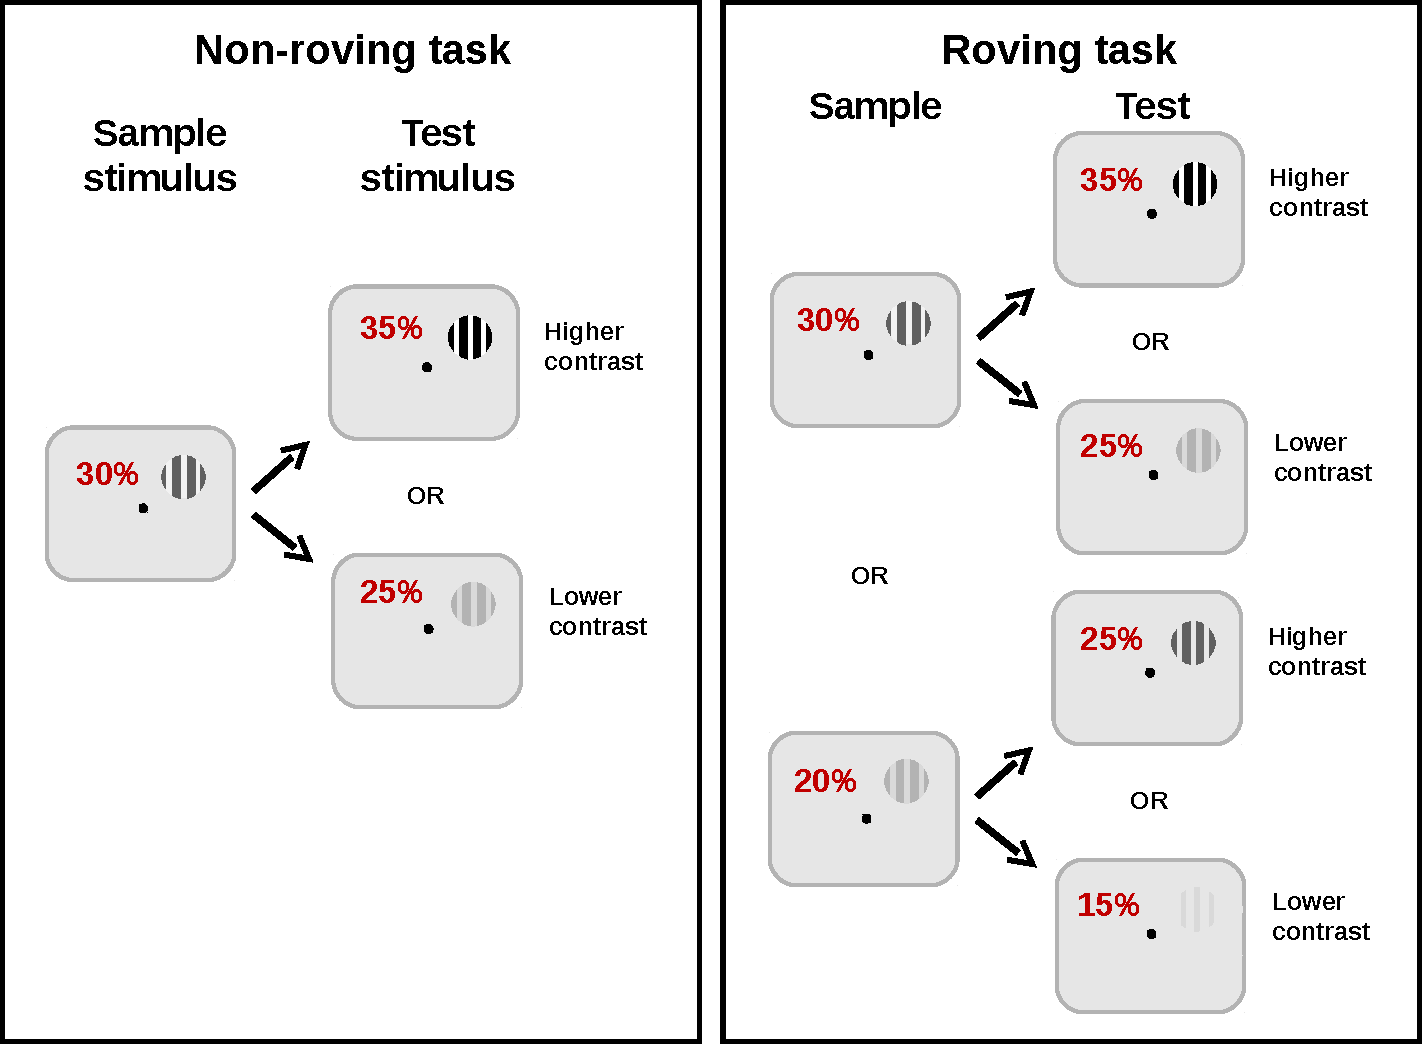
\includegraphics[width=0.8\linewidth]{figs/task/PLtask2.pdf}
\end{center}
\caption{The experimental task during both the non-roving and roving stages.
The analysis contained in this report concerns only the first, non-roving, stage.}
\label{fig:pltask2}
\end{figure}

% \begin{figure}[htbp]
% \begin{center}
% 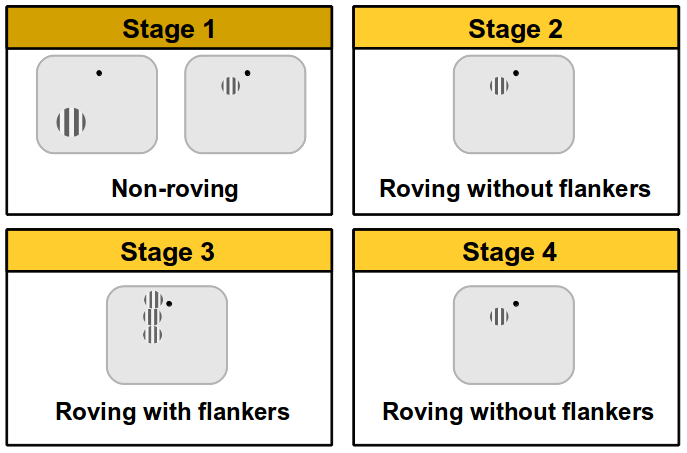
\includegraphics[width=0.8\linewidth]{figs/task/PLtask3.png}
% \end{center}
% \caption{The experiment was composed of 4 stages.
% In this analysis, we are concerned only with the first stage.}
% \label{fig:pltask3}
% \end{figure}

In this study, we will focus on analysing data from the non-roving perceptual learning task as described above.
However, it should be noted that once the animals had completed the non-roving stage of the experiment, they progressed to further stages involving a roving task.
In the roving task, the sample contrast was chosen at random with $C_\text{sample} \in \{20, 30, 40\}\%$.
Subsequently, once the test stimulus had been shown and the targets appeared, the animal was tasked with responding by comparing the test contrast to whichever sample contrast was presented on that particular trial.
During this task, the test contrast would be selected from a set of 12 contrasts specific to each of the three sample stimuli, such that 6 test stimuli were higher and 6 lower in contrast than the sample.
The difference between the non-roving and roving stages is illustrated in \autoref{fig:pltask2}.
%
% One small inconsistency in the experimental setup is that for \ac{M1} during the \ac{V4}-based task, the inter-stimuli wait was chosen randomly as $t_3 \in [x,y]ms$.
% For later experiments, including the \ac{V1} recordings for \ac{M1} and both \ac{V4} and \ac{V1} recordings for \ac{M2}, the inter-stimuli wait was fixed at $t_3 = z ms$.

As mentioned in \autoref{sec:bgpl}, some previous research has found flankers around the stimuli are necessary to induce perceptual learning.
During this experiment, the researchers found flankers were not necessary for perceptual learning during the first stage, but to subsequently learn to the roving task, flankers around the stimuli were necessary.

% A related experiment to investigate which neural receptors are important for perceptual learning to take place has been undertaken on a third monkey.
% This monkey, Frank, has been exposed to neuropharmacological agents to see how they affect perceptual learning; the two agents used are the NMDA-receptor antagonist APV, and the muscarinic and nicotinic receptor antagonist scopolamine.
